\documentclass[letterpaper,twocolumn,10pt]{article}
\usepackage{usenix-2020-09}
\usepackage{booktabs}
\usepackage{tabularx}
\usepackage{enumitem}
\usepackage{amsmath}
\usepackage{amssymb}
\usepackage{graphicx}
\usepackage{subcaption}
\newcommand{\code}[1]{\texttt{\small #1}}
%-------------------------------------------------------------------------------
\begin{document}
%-------------------------------------------------------------------------------
\date{}
\title{\Large \bf Cache Eviction on Public-Records APIs:\\
Workload Shape and Cost Attribution Decide the Policy}
\author{
{\rm Mira Yu}\\
Harvard University \\
CS 2640: Modern Storage Systems
}
\maketitle
%-------------------------------------------------------------------------------
\begin{abstract}
%-------------------------------------------------------------------------------
Which cache eviction policy wins on public-records APIs? The
actual answer depends on what the operator is paying for.
Public-records APIs (Congress.gov, CourtListener) are rate-limited
at the origin ($\sim 5{,}000$ req/hr), have no per-byte charge,
span $335\times$ size variance in a single namespace, and are
TTFB-dominated ($\sim 358$\,ms p50). Object-miss is the deployment
cost. Byte-miss is not. That attribution flips the post-2020
``size-aware-is-dead'' trend
(Caffeine~\cite{caffeine2024}, S3-FIFO~\cite{yang2023fifo},
SIEVE~\cite{zhang2024sieve}).
On two real traces with 5-seed sweeps over four $\alpha$, four cache
fractions, and ten policies (LRU, FIFO, CLOCK, S3-FIFO, SIEVE,
W-TinyLFU, GDSF, GDSF-Cost, LHD-Lite, LHD-Full), the object-miss
winner depends on workload shape. \textbf{GDSF wins on Court
(heavy-tail size)} at $\code{cache\_frac} \geq 0.01$, $3$--$9$\,pp
over W-TinyLFU at $0.01$ and $4$--$21$\,pp at $0.05$. W-TinyLFU
takes the smaller caches ($\leq 0.005$). \textbf{LHD-Full wins on
Congress (light-tail size)} at $\alpha = 0.6$ ($1.8$\,pp over GDSF,
$n{=}20$, Welch $p<10^{-4}$), where its residual-reuse-distance
signal beats GDSF's size-priority. The $\alpha=0.8$ cell is a
statistical tie at $n{=}20$ ($0.2$\,pp gap, $p=0.65$). Three
controls narrow the SIEVE-vs.-W-TinyLFU gap on Court to size-outlier
rejection, not frequency-gradient capture. LHD-Full is
Pareto-dominated by the GDSF--W-TinyLFU convex hull on Court ($7/8$
deployment-relevant cells) but anchors the object-miss frontier on
Congress at $\alpha = 0.6$.
For byte-priced backends (S3 egress) the verdict flips to W-TinyLFU
on Court and SIEVE on Congress: same measurements, opposite winner.
Picking a metric without naming the cost model picks the policy by
accident.
\end{abstract}
%-------------------------------------------------------------------------------
% Hero figure (full-width, two-column-spanning)
%-------------------------------------------------------------------------------
\begin{figure*}[t]
\centering
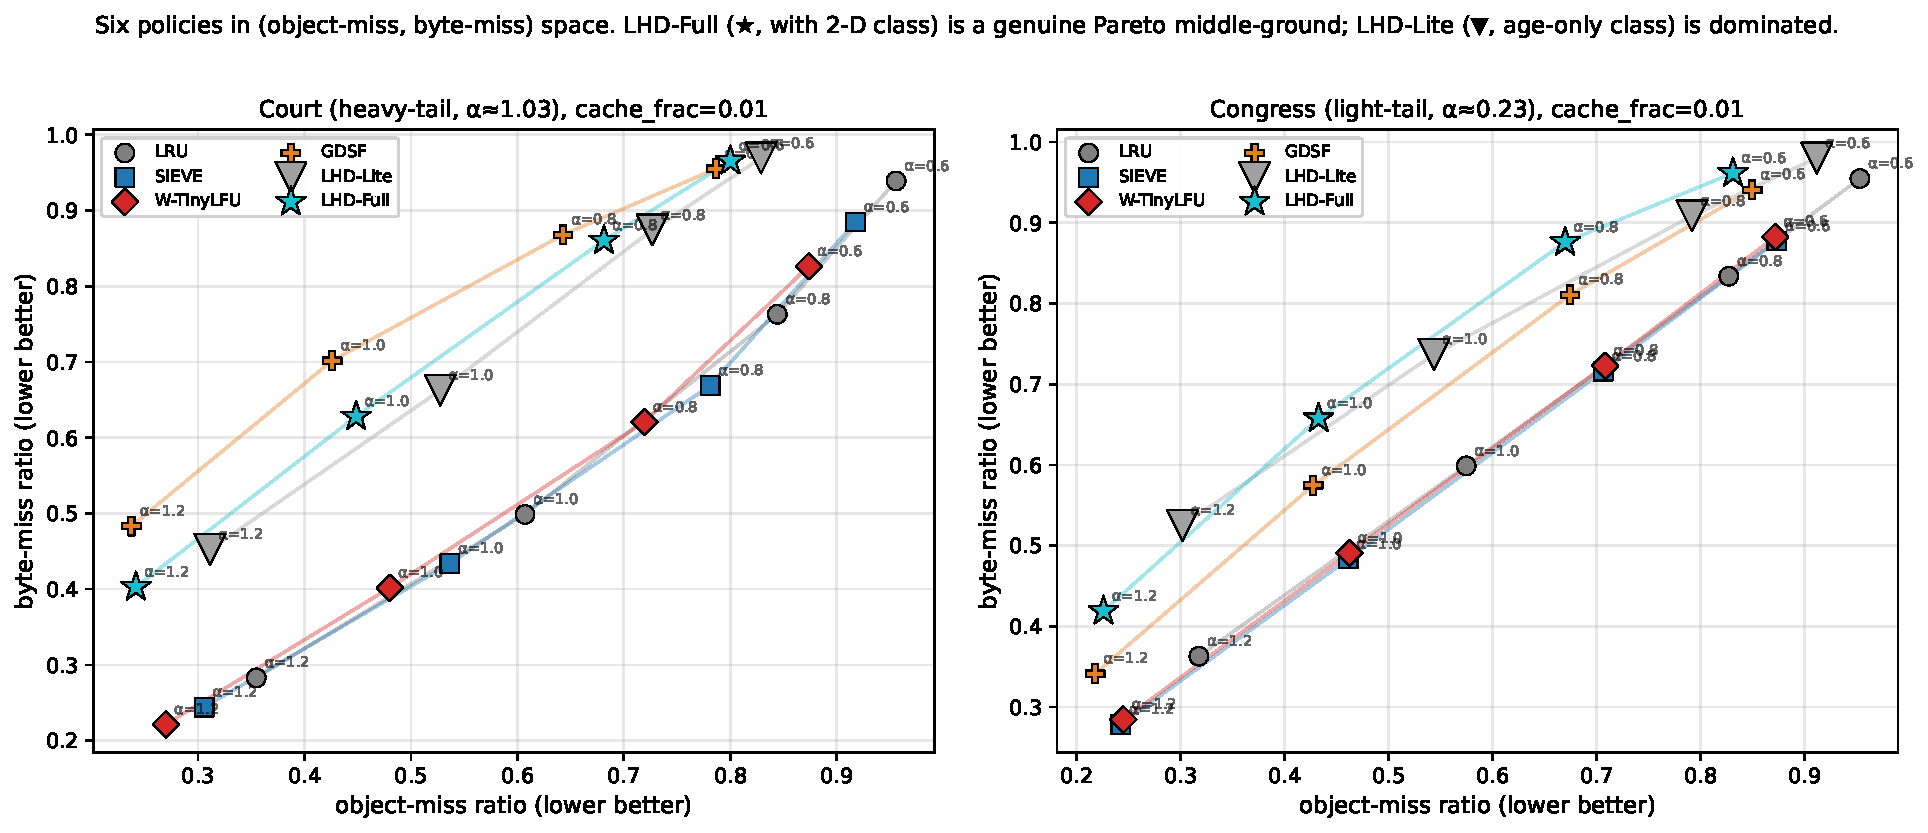
\includegraphics[width=0.75\textwidth]{figures/obj_vs_byte_lhdfull.pdf}
\caption{Six policies in (object-miss, byte-miss) space at
$\code{cache\_frac} = 0.01$, four $\alpha$ overlays per workload.
GDSF anchors the low-object-miss frontier. W-TinyLFU anchors the
low-byte-miss frontier. The two are not co-optimizable, and which
axis is the deployment cost depends on who pays (\S\ref{sec:weighted}).}
\label{fig:headline}
\end{figure*}
%-------------------------------------------------------------------------------
\section{Introduction}\label{sec:intro}
%-------------------------------------------------------------------------------
The TinyLFU paper~\cite{einziger2017tinylfu} argued that frequency
tracking would dominate recency-only eviction. The post-2020
literature (Caffeine~\cite{caffeine2024}, S3-FIFO~\cite{yang2023fifo},
SIEVE~\cite{zhang2024sieve}) has implicitly accepted that framing
while moving away from size-aware policies. The broader 2000s
adaptive-cache work (ARC~\cite{megiddo2003arc}) is recency+frequency
and is also not size-aware.

GDSF~\cite{cherkasova1998gdsf} was designed for 1998 web proxies
where bandwidth dominated cost; the post-2020 KV/CDN literature
moved away from per-byte attribution because in-cluster caches
don't pay for bytes. Rate-limited public APIs (citizen-tech,
monetary-quota services, scrape-respectful clients) revive the
per-request cost model on a workload class the cache literature
has not characterized.

I collected two real public-records API traces (Congress.gov,
CourtListener), ran a 5-seed comparison of ten policies including
GDSF and LHD~\cite{beckmann2018lhd}, and tabulated \emph{both}
object-miss and byte-miss for every cell. The headline result is
that GDSF wins object-miss on Court at deployment-relevant cache
fractions, LHD-Full wins on Congress at $\alpha = 0.6$ ($1.8$\,pp
over GDSF, $n{=}20$) and ties GDSF at $\alpha = 0.8$ ($n{=}20$),
and W-TinyLFU wins byte-miss universally on Court. The pattern only
comes out the cost model is made explicit (\S\ref{sec:weighted})
rather than picked a priori by metric choice.
\paragraph{Why public-records APIs are a distinct workload class.}
Most cache-policy benchmark papers treat ``the workload'' as
interchangeable Zipf parameters. What differs across CDN, key-value,
and storage benchmarks is mostly $\alpha$ and the size distribution.
Public-records APIs are different in five concrete ways that change
that:
\begin{enumerate}[leftmargin=*,itemsep=1pt,topsep=2pt]
  \item \textbf{The origin is rate-limited, not bandwidth-billed.}
    Congress.gov and CourtListener publish hard quotas
    ($\sim 5{,}000$ req/hr), and breaches return 429s rather than
    overage charges. The operator's binding cost is requests
    issued to origin, not bytes transferred. This collapses the
    object-miss/byte-miss tradeoff in favor of object-miss
    (\S\ref{sec:weighted}).
  \item \textbf{Heavy size variance inside one namespace.}
    A single CourtListener \texttt{/opinion/} prefix returns both
    $200$\,B metadata stubs and $462$\,KB full-text opinions
    ($335\times$ ratio, Table~\ref{tab:workload}). Most cache
    benchmark traces are size-uniform (key-value) or size-binned
    (video chunks). The same key prefix in this workload spans the
    full size range.
  \item \textbf{TTFB-dominated origin response} ($358$\,ms combined
    $p_{50}$). Cost of a miss is whether-you-hit, not transfer time
    making latency $\approx$ object-miss $\times \, L_{\text{origin}}$
    tight up to $\sim 100$\,KB sizes (\S\ref{sec:weighted}).
  \item \textbf{The cache is the only operator lever.} A private
    operator can't scale, renegotiate, or bypass the public origin.
    Cache hit rate directly bounds simultaneous users.
  \item \textbf{Catalog-then-deepdive access.} Sessions enumerate
    catalogs (many low-freq items) then drill into specific
    records (few high-freq items). On Court, $25\%$ of requests
    revisit a prior key, the top $10\%$ of keys absorb $32\%$ of
    traffic, and one document is fetched $273$ times
    ($\alpha \approx 1.03$).
\end{enumerate}
Traits 1 and 3 together make object-miss the unique cost. Trait
2 makes size-aware admission valuable, 4 makes the result
deployable, and 5 gives the high-$\alpha$
structure caching needs to work at all. None of these are unique
individually. CDN traces have heavy tails, and key-value caches have
rate-limit-like SLOs. Public-records APIs combine all five, and
that combination is unique.
\paragraph{Note on trace.} Both real traces are dominated by one-hit
wonders ($\S$\ref{sec:methodology}), so the policy comparison runs
against a controlled Zipf overlay on the real key set (real keys,
real sizes, resampled popularity ranks). The key/size distributions
carry the workload-class signal, and the popularity is the
controlled variable.
%-------------------------------------------------------------------------------
\section{Related Work}\label{sec:related}
%-------------------------------------------------------------------------------
\paragraph{Modern cache eviction.} The post-2020 wave of
S3-FIFO~\cite{yang2023fifo}, SIEVE~\cite{zhang2024sieve}, and
Caffeine's W-TinyLFU~\cite{caffeine2024} converges on
recency/frequency signals over size-aware admission, building on
TinyLFU~\cite{einziger2017tinylfu} and the earlier
ARC~\cite{megiddo2003arc}. Each evaluation implicitly fixes its cost
model by metric choice. SIEVE and S3-FIFO target object-miss for
KV/web. LHD~\cite{beckmann2018lhd} targets byte-miss for CDN.
GDSF~\cite{cherkasova1998gdsf} sits outside this trend and has not
appeared in the post-2020 comparison set, which is why I revisit it under workload-class-specific cost attribution.
\paragraph{Trace characterization.} Most published cache benchmarks
treat workload as interchangeable Zipf parameters with optional size
binning. CDN traces (Akamai, Wikipedia) are heavy-tailed in
popularity but typically size-binned by content type. KV traces
(Twitter, Memcached production) are size-uniform within a namespace.
Heavy size variance within a single key prefix ($335\times$ on a
single CourtListener URL prefix) is rare in the published trace
literature, and that's what drives GDSF's win here.
\paragraph{Cache simulators.} The CMU CORGI/LHD reference
implementation is the canonical LHD codebase. I validate
against the LHD paper's Memcached comparison (\S\ref{sec:methodology},
$13$--$18$\,pp over LRU on a synth-faithful trace) but I didn't yet
run a byte-for-byte CORGI comparison (which could be future work, see
\S\ref{sec:conclusion}). SHARDS~\cite{waldspurger2015shards} provides
MRC sampling, used here for self-convergence validation
(\S\ref{sec:ablations}).
\paragraph{Cost-aware evaluation.} GDSF~\cite{cherkasova1998gdsf}
is itself cost-aware (priority $H = f \cdot c / s + L$). The
cost-aware literature historically jointly optimizes hit-rate and
bandwidth for web proxies. My contribution is not new
policy design but cost-attribution-driven policy selection.
When the operator's binding cost is requests-to-origin (rate-limited
APIs), the right policy differs from the byte-priced default, and
that choice deserves to be named in the cost model.
\paragraph{API gateway caching.} Production API gateways (Kong,
Cloudflare Workers, AWS API Gateway) ship LRU/TTL by default.
Cache-policy choice for rate-limited public APIs is largely
undocumented in the academic literature, which is the gap I address.
%-------------------------------------------------------------------------------
\section{Workloads and Methodology}\label{sec:methodology}
%-------------------------------------------------------------------------------
\begin{figure*}[t]
\centering
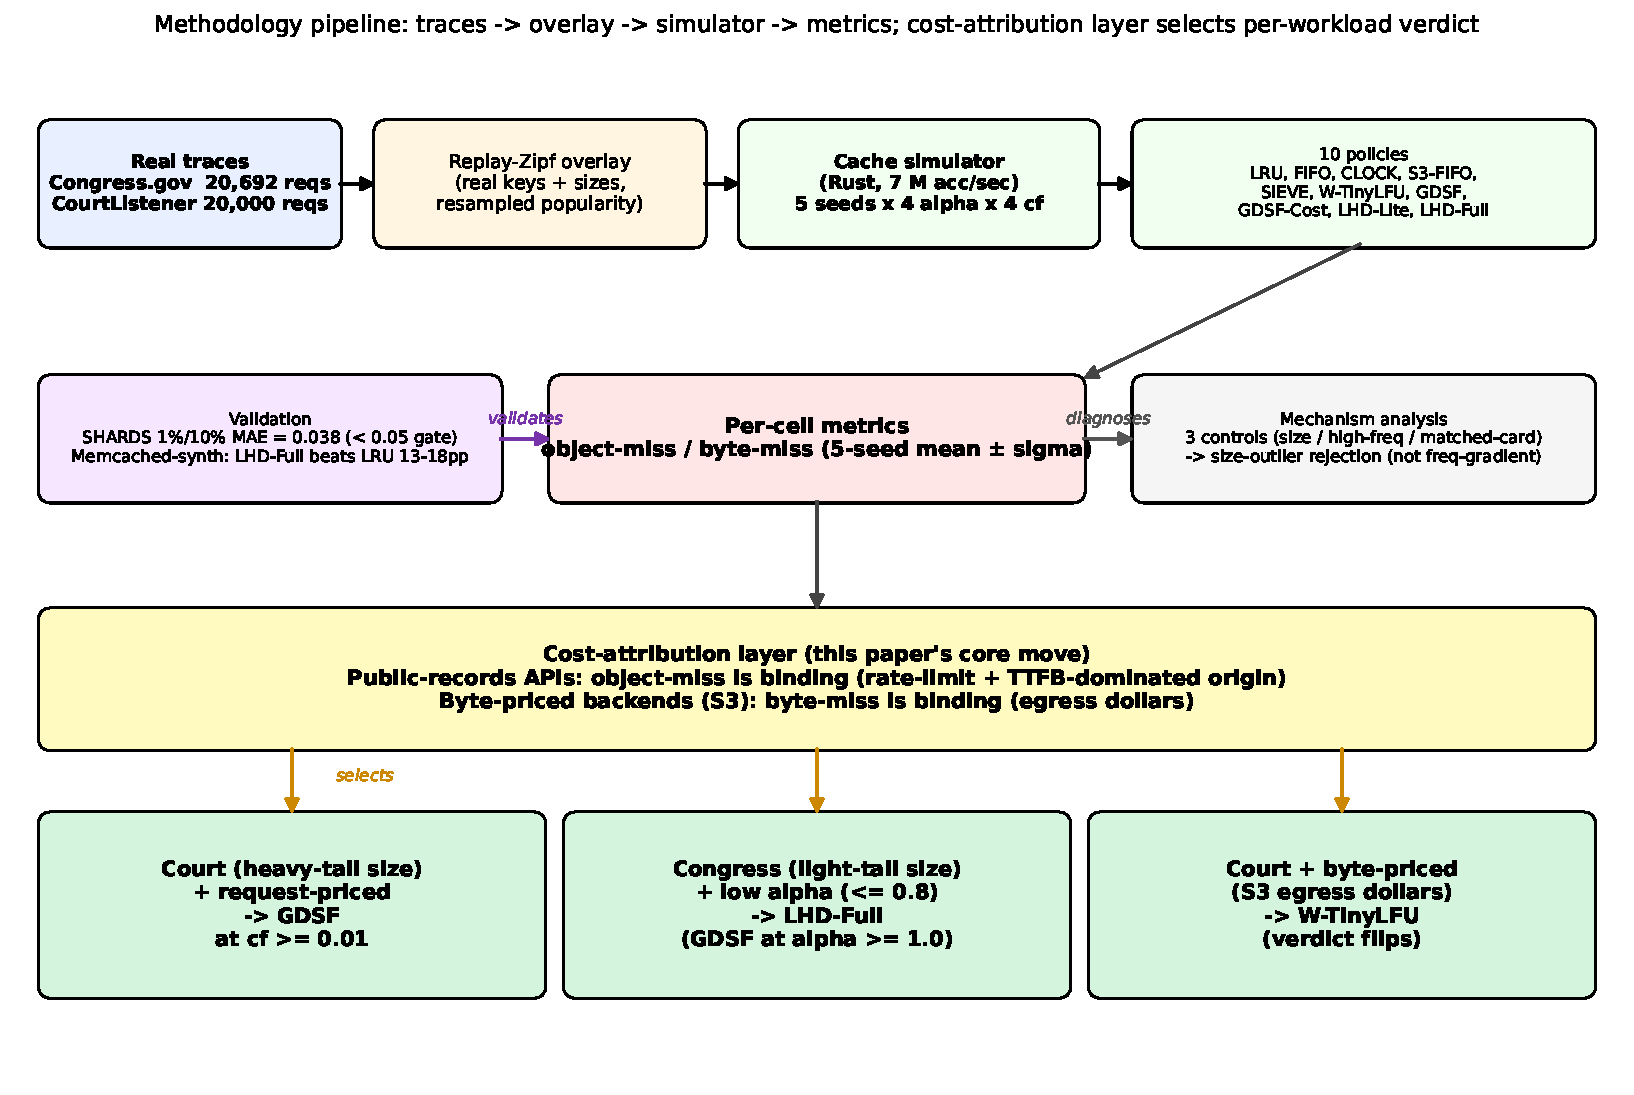
\includegraphics[width=0.92\textwidth]{figures/methodology_diagram.pdf}
\caption{Methodology pipeline. Real traces feed a Zipf-overlay
preprocessor, then a Rust simulator runs ten policies under a
$5 \times 4 \times 4$ sweep, validated by SHARDS and a
Memcached-faithful synth. The cost-attribution layer selects a
deployment verdict from the same per-cell metrics.}
\label{fig:methodology}
\end{figure*}
\begin{table*}[t]
\centering
\footnotesize
\renewcommand{\arraystretch}{0.95}
\begin{tabularx}{\textwidth}{@{}lXX@{}}
\toprule
\textbf{Metric} & \textbf{Congress.gov} & \textbf{CourtListener} \\
\midrule
Total requests / unique keys & $20{,}692$ / $18{,}970$ & $20{,}000$ / $15{,}018$ \\
Zipf $\alpha$ (Clauset MLE)~\cite{clauset2009powerlaw} & $0.231$ & $1.028$ \\
One-hit-wonder ratio (10\% rolling window) & $0.989$ & $1.000$ \\
Median / max object size (B) & $231$ / $6{,}700$ & $1{,}381$ / $\mathbf{462{,}490}$ \\
Max / median ratio  & $29\times$ & $\mathbf{335\times}$ \\
Origin $p_{50}$ response (ms) & $321$ & $383$ \\
Working set (bytes) & $14.5$\,MB & $59.6$\,MB \\
\bottomrule
\end{tabularx}
\caption{Side-by-side trace characterization. The bold rows (Court's
high $\alpha$ and $335\times$ size ratio) drive the policy gap in
$\S$\ref{sec:gdsf}--$\S$\ref{sec:mechanism}.}
\label{tab:workload}
\end{table*}
\paragraph{Where each policy appears.} Focal object-miss/byte-miss sweep
(Table~\ref{tab:focal-court}): SIEVE, W-TinyLFU, GDSF, LHD-Full.
Hero figure adds LRU and LHD-Lite. \S\ref{sec:ablations} tests
S3-FIFO, SIEVE$\pm$visited-bit, W-TinyLFU$\pm$Doorkeeper. FIFO,
CLOCK, and GDSF-Cost run in the synthetic $1$\,M-request sweep
behind \S\ref{sec:mechanism}.
\paragraph{Trace collection.} Congress.gov v3 REST at $1.2$\,s
pacing sweeping \texttt{/bill/}, \texttt{/amendment/},
\texttt{/vote/}. CourtListener REST v4 at $0.8$\,s base $+ 0.4$\,s
jitter, $80/20$ metadata vs full-text. Both are client-generated
random queries against cataloged keys, since no production
user-traffic capture exists. Rate-limit-bounded at $\sim 4500$/hour
and $\sim 5000$/hour respectively.
\paragraph{Why $20$\,K requests.} The policy-relevant
signal here is the size and key distribution, both stationary by
construction. Working-set bytes converge by $\sim 5$\,K requests,
and Clauset-MLE $\alpha$ on Court is stable to $\pm 0.02$ between
$10$\,K and $20$\,K. I re-ran borderline cells at $n{=}20$ seeds
(\S\ref{sec:gdsf}). Court's deployment-relevant gaps ($3$--$9$\,pp)
are an order of magnitude above any plausible trace-size noise.
\paragraph{Replay-Zipf overlay.} The OHW dominance ($\geq 0.989$)
on both raw traces means a direct replay collapses every policy to
FIFO. I overlaid a controlled Zipf popularity distribution on the
real key set (real keys, real sizes, resampled popularity ranks).
The distribution is the controlled variable. The keys and sizes are
real.
\paragraph{GDSF / LHD implementation.}
GDSF~\cite{cherkasova1998gdsf} maintains $H = f \cdot c / s + L$ per
item, evicting $\arg\min H$ via an $O(\log n)$ min-heap with lazy
stale-entry deletion. I tested both unit-cost ($c=1$) and an
empirical linear cost fit ($c = 530 + 0.00254 \cdot
\text{size}_{\text{B}}$). The two agree within $0.5$\,pp because
size variation ($335\times$) dominates cost variation
($3.2\times$). I implement LHD~\cite{beckmann2018lhd} per NSDI'18
\S 4 in two versions: \textbf{LHD-Lite} (single-class, age only)
and \textbf{LHD-Full} (2-D classes age$\times$freq, $16$ log-spaced
age bins $\times\,4$ freq bins, EWMA-decayed histograms, $K=64$
candidate sampling). LHD-Lite is dominated by every modern policy.
LHD-Full wins on Congress at $\alpha=0.6$ (\S\ref{sec:gdsf}).
\textbf{Implementation validation:} on a Memcached-faithful synth
($200$K objects, $\alpha=0.9$, log-normal sizes
$\mu=6.5,\sigma=1.5$), LHD-Full beats LRU by $13$--$18$\,pp and
matches GDSF within $\pm 0.5$\,pp, reproducing NSDI'18's primary
claim. So Court Pareto-domination by GDSF (\S\ref{sec:weighted}) is
 workload-class divergence.
%-------------------------------------------------------------------------------
\section{Per-Metric Results}\label{sec:gdsf}
%-------------------------------------------------------------------------------
Focal sweep: $5$ seeds $\times$ $4$ alphas $\times$ $4$ cache fractions,
both workloads, both metrics. All 16 Court cells in
Table~\ref{tab:focal-court}; Congress slice in
Table~\ref{tab:focal-congress}. I didn't rerun Court at $20$ seeds
because the deployment-relevant gaps ($3$--$9$\,pp at
$\code{cf} \geq 0.01$) are outside any plausible seed-$\sigma$
reversal. Congress object-miss was re-run at $n{=}20$ to power the
small-effect cells.
\begin{table*}[t]
\centering
\footnotesize
\renewcommand{\arraystretch}{0.95}
\begin{tabularx}{\textwidth}{@{}llXXXX@{}}
\toprule
$\alpha$ & cf & SIEVE & W-TinyLFU & GDSF & LHD-Full \\
\midrule
$0.6$ & $0.001$ & $0.992 / 0.995$ & $\mathbf{0.942}$ / $\mathbf{0.975}$ & $0.988 / 0.996$ & $0.987 / 0.996$ \\
$0.6$ & $0.005$ & $0.960 / 0.970$ & $\mathbf{0.891}$ / $\mathbf{0.936}$ & $0.921 / 0.979$ & $0.918 / 0.980$ \\
$0.6$ & $0.01$  & $0.918 / 0.885$ & $0.874 / \mathbf{0.826}$            & $\mathbf{0.787}$ / $0.955$ & $0.800 / 0.966$ \\
$0.6$ & $0.05$  & $0.747 / 0.700$ & $0.730 / \mathbf{0.699}$            & $\mathbf{0.518}$ / $0.863$ & $0.550 / 0.849$ \\
$0.8$ & $0.001$ & $0.949 / 0.969$ & $\mathbf{0.836}$ / $\mathbf{0.927}$ & $0.938 / 0.974$ & $0.938 / 0.974$ \\
$0.8$ & $0.005$ & $0.860 / 0.891$ & $\mathbf{0.741}$ / $\mathbf{0.848}$ & $0.805 / 0.919$ & $0.802 / 0.919$ \\
$0.8$ & $0.01$  & $0.781 / 0.669$ & $0.719 / \mathbf{0.621}$            & $\mathbf{0.643}$ / $0.868$ & $0.681 / 0.861$ \\
$0.8$ & $0.05$  & $0.549 / 0.477$ & $0.542 / \mathbf{0.476}$            & $\mathbf{0.379}$ / $0.613$ & $0.409 / 0.651$ \\
$1.0$ & $0.001$ & $0.813 / 0.880$ & $\mathbf{0.641}$ / $\mathbf{0.830}$ & $0.793 / 0.894$ & $0.791 / 0.891$ \\
$1.0$ & $0.005$ & $0.670 / 0.733$ & $\mathbf{0.511}$ / $\mathbf{0.708}$ & $0.601 / 0.776$ & $0.599 / 0.776$ \\
$1.0$ & $0.01$  & $0.537 / 0.434$ & $0.480 / \mathbf{0.402}$            & $\mathbf{0.426}$ / $0.702$ & $0.449 / 0.628$ \\
$1.0$ & $0.05$  & $0.317 / 0.265$ & $0.309 / \mathbf{0.264}$            & $\mathbf{0.217}$ / $0.348$ & $0.230 / 0.395$ \\
$1.2$ & $0.001$ & $0.629 / 0.748$ & $\mathbf{0.445}$ / $\mathbf{0.706}$ & $0.607 / 0.766$ & $0.605 / 0.762$ \\
$1.2$ & $0.005$ & $0.466 / 0.574$ & $\mathbf{0.297}$ / $\mathbf{0.559}$ & $0.412 / 0.611$ & $0.412 / 0.612$ \\
$1.2$ & $0.01$  & $0.306 / 0.244$ & $0.270 / \mathbf{0.221}$            & $\mathbf{0.242}$ / $0.483$ & $0.242 / 0.403$ \\
$1.2$ & $0.05$  & $0.145 / 0.122$ & $0.140 / \mathbf{0.121}$            & $\mathbf{0.099}$ / $0.167$ & $0.104 / 0.195$ \\
\bottomrule
\end{tabularx}
\caption{Court, all 16 cells: object-miss / byte-miss, $5$-seed mean.
\textbf{Bold} = per-cell metric winner. \emph{Object-miss winner counts:}
GDSF $8$ (cf $\geq 0.01$), W-TinyLFU $8$ (cf $\leq 0.005$). \emph{Byte-miss
winner counts:} W-TinyLFU $16/16$. The byte-miss gap ranges $4$--$30$\,pp.}
\label{tab:focal-court}
\end{table*}
\paragraph{Why GDSF wins object-miss / W-TinyLFU wins byte-miss.}
GDSF's priority $H = f \cdot c / s + L$ favors small items by $1/s$
(with $c=1$). A $200$\,B metadata stub raises $H$ by
$5{\times}10^{-3}$ per access. The $462$\,KB Court opinion raises it
by $2.2{\times}10^{-6}$, $2{,}300\times$ less. The opinion sits at
$H \approx L$ regardless of frequency and is evicted first, so GDSF
caches more items per byte (low object-miss) and re-fetches
the opinion on every visit (high byte-miss). W-TinyLFU's CMS-based
admission picks on access count alone. Once the opinion reaches high
CMS it stays cached (low byte-miss), while each of the $\sim 230$
small items it displaces must be re-fetched (higher object-miss).
The two policies anchor opposite ends of the object-miss/byte-miss
Pareto frontier, and neither dominates on both axes.
\begin{figure*}[t]
\centering
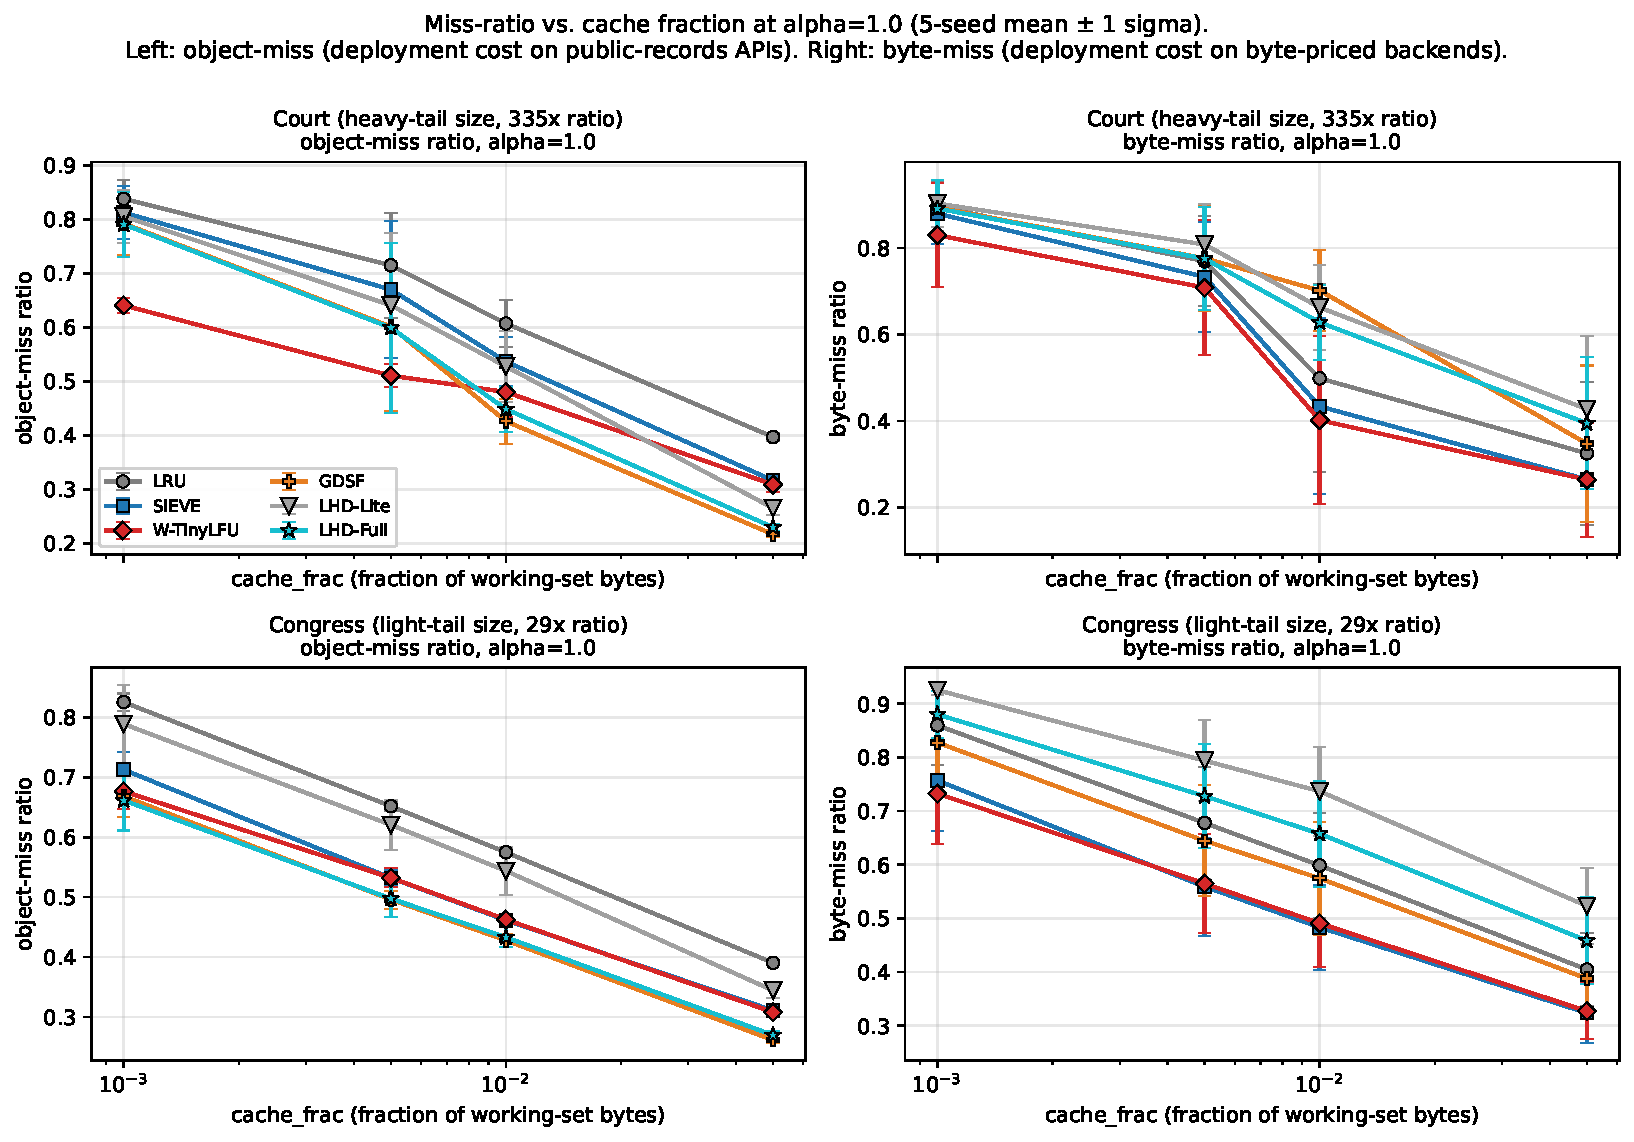
\includegraphics[width=0.95\textwidth]{figures/miss_vs_cf.pdf}
\caption{Miss-ratio vs.\ cache fraction at $\alpha = 1.0$, $5$-seed
mean $\pm 1\sigma$. \textbf{Court (top):} W-TinyLFU leads object-miss
at $\code{cf} \leq 0.005$; GDSF and LHD-Full overtake at $\geq 0.01$
(the Table~\ref{tab:focal-court} crossover, plotted). \textbf{Congress
(bottom):} GDSF and LHD-Full are visually indistinguishable on
object-miss; SIEVE/W-TinyLFU lead byte-miss.}
\label{fig:miss-vs-cf}
\end{figure*}
\paragraph{Congress focal.} On Congress, the object-miss winner
depends on $\alpha$ (Figure~\ref{fig:congress-alpha}):
\begin{table}[t]
\centering
\footnotesize
\renewcommand{\arraystretch}{0.9}
\begin{tabularx}{\columnwidth}{@{}lXXXXl@{}}
\toprule
$\alpha$ & SIEVE & W-TLFU & GDSF & LHD-F & winner \\
\midrule
$0.6$ & $0.875$ & $0.872$ & $0.850$ & $\mathbf{0.832}$ & LHD-F \\
$0.8$ & $0.707$ & $0.709$ & $0.674$ & $0.672$ & tie \\
$1.0$ & $0.460$ & $0.464$ & $\mathbf{0.426}$ & $0.436$ & GDSF \\
$1.2$ & $0.244$ & $0.246$ & $\mathbf{0.218}$ & $0.226$ & GDSF \\
\bottomrule
\end{tabularx}
\caption{Congress object-miss at $\code{cf} = 0.01$, $20$-seed
mean (re-run from the original $5$-seed sweep to close the rigor
gap on the $\alpha=0.8$ cell). Welch $t$ on LHD-Full $-$ GDSF
at $n{=}20$:
\textbf{$\alpha=0.6$:} $-1.82$\,pp, $p<10^{-4}$ (LHD-F).
\textbf{$\alpha=0.8$:} $-0.21$\,pp, $p=0.65$ (tie; the $5$-seed
$0.5$\,pp LHD-F lead does not survive).
\textbf{$\alpha=1.0$:} $+1.02$\,pp, $p=0.015$ (GDSF).
\textbf{$\alpha=1.2$:} $+0.83$\,pp, $p=0.007$ (GDSF). All three
non-tie cells are significant at $0.05$.}
\label{tab:focal-congress}
\end{table}
\begin{figure}[t]
\centering
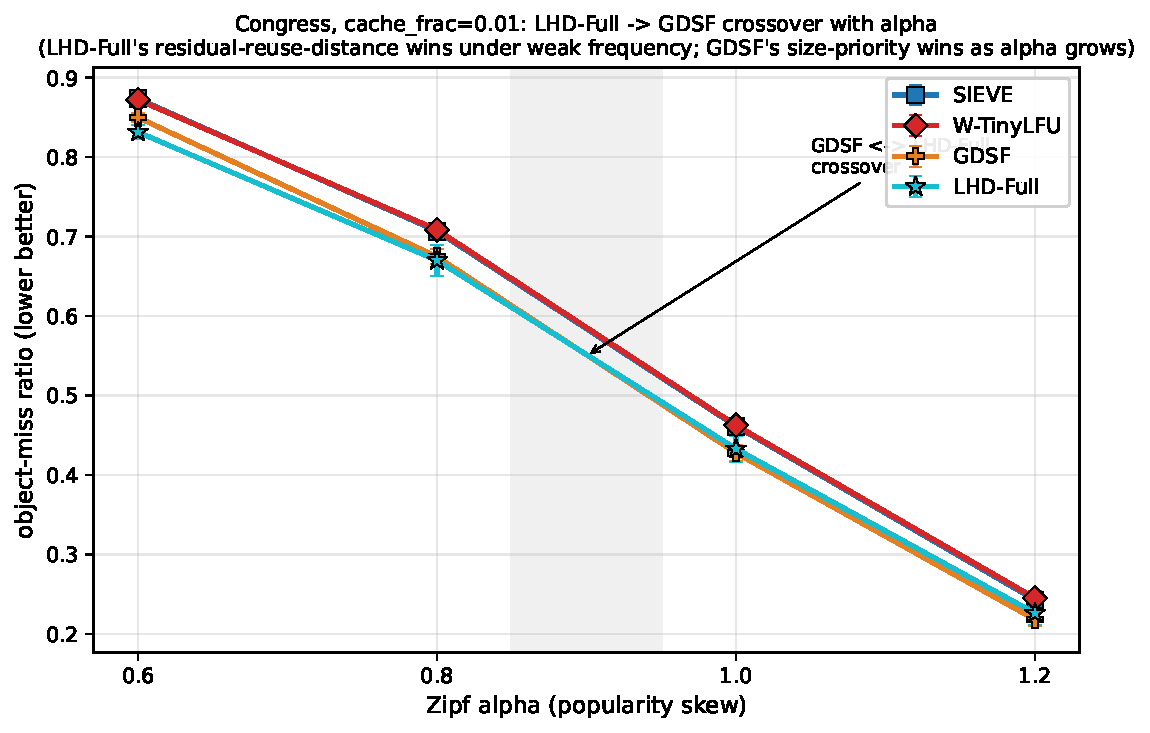
\includegraphics[width=0.95\columnwidth]{figures/congress_alpha_crossover.pdf}
\caption{Congress object-miss vs.\ $\alpha$ at $\code{cf}=0.01$
(Table~\ref{tab:focal-congress} plotted, $20$-seed mean).
\textbf{20-seed re-run} confirms LHD-Full's lead at $\alpha=0.6$
($1.8$\,pp, $p<10^{-4}$); the $\alpha=0.8$ LHD-F-vs-GDSF gap is a
statistical tie ($0.2$\,pp, $p=0.65$); GDSF takes over at
$\alpha \geq 1.0$ ($p \leq 0.015$). SIEVE and W-TinyLFU are
indistinguishable (\S\ref{sec:mechanism}, $p \geq 0.20$ at $20$
seeds).}
\label{fig:congress-alpha}
\end{figure}
\paragraph{LHD-Full's actual position.} LHD-Full anchors the
object-miss frontier on Congress at $\alpha = 0.6$ (and ties GDSF at
$\alpha = 0.8$ at $n{=}20$; see Table~\ref{tab:focal-congress} and
Figure~\ref{fig:congress-alpha}), but on Court it is dominated by
the GDSF--W-TinyLFU convex hull at deployment-relevant cache
fractions (per-cell breakdown in \S\ref{sec:weighted}). The 2-D
class implementation closes a $7$\,pp gap vs.\ LHD-Lite at
$(\alpha, \text{cf}) = (1.0, 0.01)$. Per
\S\ref{sec:methodology}'s Memcached-faithful validation, the
residual Court-side gap is workload-class divergence, not
implementation incompleteness. Throughput is $\sim 500$\,K
acc/sec, $14\times$ slower than W-TinyLFU.
%-------------------------------------------------------------------------------
\section{Cost Attribution}\label{sec:weighted}
%-------------------------------------------------------------------------------
\noindent Pick the metric that matches the operator's binding
cost. The two metrics in $\S$\ref{sec:gdsf} disagree. Most cache
benchmarks resolve this by silently picking object-miss
(Memcached-style) or byte-miss (CDN-style). I make the cost model
explicit and use it to pick a Pareto-frontier point.
\paragraph{Worked example: a $5.4$\,pp object-miss saving in
operator units.} Take the GDSF-vs.-W-TinyLFU gap at $(\alpha,
\text{cf}) = (1.0, 0.01)$ on Court: $0.480 \to 0.426 = 5.4$\,pp.
(i) Rate-limit headroom. Origin reqs/hr $=
\text{object-miss} \cdot R_{\text{offered}}$. At a hypothetical
$18{,}000$ reqs/hr offered load ($3.6\times$ the single-key quota,
a sensitivity-analysis point not a measured value), GDSF issues
$7{,}668$ origin reqs/hr vs.\ W-TinyLFU's $8{,}640$, a $972$
req/hr saving. Against the linearly-scaling $5{,}000$/hr quota,
that's the difference between needing $1.7$ vs.\ $1.9$ API keys
(one extra concurrent user before the operator provisions another
credentialed pool). At $50{,}000$/hr the saving is $2{,}700$/hr,
half a quota slot.
(ii) End-user latency. Per-request latency at
$L_{\text{origin}} = 383$\,ms is $233$\,ms under LRU (the gateway
default), $184$\,ms under W-TinyLFU, and $163$\,ms under GDSF
(Table~\ref{tab:lat}). GDSF saves $\sim 69$\,ms/request vs.\ LRU
and $\sim 21$\,ms vs.\ W-TinyLFU. Treating the $20$\,K-request
trace as a one-day proxy, that's $\sim 23$ and $\sim 7$ minutes
of aggregate user wait eliminated.
(iii) Byte-miss is zero deployment cost here. GDSF's
byte-miss is $30$\,pp worse than W-TinyLFU's ($0.702$ vs.\
$0.402$). For a public-records operator, that costs zero dollars
and zero rate-limit budget. Bytes don't cost the operator anything.
Origin requests do, and the quota is binding.
\paragraph{Public-records cost model.} The operator pays for three
things: requests issued to origin (rate-limit budget), end-user
latency (proportional to object-miss given TTFB-dominated origin),
and origin server load (reputational, since both APIs publish
acceptable-use policies). All three scale with object-miss, not
with bytes. Byte-miss isn't a deployment cost on
this workload class.
\paragraph{Latency $\approx$ object-miss $\cdot L_{\text{origin}}$
holds at realistic throughputs.} For a steady-state cache,
$\mathbb{E}[\text{lat}] = H \cdot L_{\text{cache}} + (1-H) \cdot
L_{\text{origin}}$. Take the $462$\,KB Court outlier as worst-case
transfer: at $10$\,MB/s WAN it is $46$\,ms vs.\ $L_{\text{origin}}
= 358$\,ms ($13\%$). For typical $12$\,KB objects, transfer is
$1.2$\,ms. The approximation holds within $5$\,pp up to
$\sim 100$\,KB. Origin TTFB is dominated by backend-database
response time. Both APIs front legacy government databases
(CourtListener built on RECAP infrastructure, Congress.gov on the
Library of Congress's record system), and neither is optimizable
from the cache layer. Table~\ref{tab:lat} translates the per-policy
object-miss into per-request latency at the Court anchor.
\begin{table}[t]
\centering
\footnotesize
\renewcommand{\arraystretch}{0.95}
\begin{tabularx}{\columnwidth}{@{}lXXX@{}}
\toprule
\textbf{Court @ cf $= 0.01$, $\alpha = 1.0$} & \textbf{obj-miss} & \textbf{lat/req (ms)} & \textbf{vs.\ no-cache} \\
\midrule
no cache  & $1.000$        & $383$ & $1.00\times$ \\
LRU       & $0.607$        & $233$ & $0.61\times$ \\
SIEVE     & $0.537$        & $206$ & $0.54\times$ \\
LHD-Lite  & $0.528$        & $203$ & $0.53\times$ \\
W-TinyLFU & $0.480$        & $184$ & $0.48\times$ \\
LHD-Full  & $0.449$        & $172$ & $0.45\times$ \\
GDSF      & $\mathbf{0.426}$ & $\mathbf{164}$ & $\mathbf{0.43\times}$ \\
\bottomrule
\end{tabularx}
\caption{Per-request latency, Court anchor $L_{\text{origin}} = 383$\,ms,
$L_{\text{cache}} = 1$\,ms. GDSF saves $\sim 21$\,ms vs.\
W-TinyLFU, $\sim 39$\,ms vs.\ LHD-Lite, and $\sim 69$\,ms vs.\
LRU.}
\label{tab:lat}
\end{table}
\paragraph{Byte-miss variance.} Byte-miss has $4$--$7\times$ the
seed-$\sigma$ of object-miss on Court (W-TinyLFU $0.402 \pm 0.241$,
std/mean $= 60\%$). A single realization either samples the heavy
outlier into cache or doesn't, and the answer moves by $\sim 30$\,pp
either way. That is why I don't decide the headline on byte-miss.
\paragraph{Why GDSF wins object-miss at mid-cache, W-TinyLFU at
small cache.} At $\code{cf} = 0.01$ on Court the byte budget is
$\sim 596$\,KB ($\sim 50$ items at $E[\text{size}]=12$\,KB, or
$\sim 430$ biased toward small). GDSF refuses to admit the
$462$\,KB document and re-fetches it on every visit, freeing room
for $\sim 230$ $2$\,KB items. W-TinyLFU's CMS admits the document
if its frequency exceeds incumbents', keeping it cached but
crowding out small items. At $\code{cf} \leq 0.005$ ($\sim 298$\,KB,
can't fit the outlier), the budget admits only the hottest items;
GDSF's size-priority then crowds out big-but-frequent items in
favor of small mid-frequency ones, hurting object-miss, and
W-TinyLFU's frequency-only admission wins. The crossover at
$\code{cf} \in [0.005, 0.01]$ is robust across $\alpha$.
\paragraph{LHD-Full is Pareto-dominated on Court where caching
matters.} At $(\alpha, \text{cf}) = (1.0, 0.01)$: GDSF $(0.426,
0.702)$, W-TinyLFU $(0.480, 0.402)$, LHD-Full $(0.449, 0.628)$.
The convex combination at byte $= 0.628$ ($t = 0.247$) gives
$\text{obj} = 0.439$, $1$\,pp better than LHD-Full at the same
byte-miss. (The hull is a theoretical bound, achievable only by
partitioning between endpoints; single-policy deployments realize
only the endpoints, which suffices here.) Per-cell
(Table~\ref{tab:lhdfull-pareto}): \textbf{Pareto-dominated in
$8/16$ Court cells} (including $7/8$ deployment-relevant cells at
$\code{cf} \geq 0.01$), by $\geq 1.3$\,pp at
$\alpha \in \{0.6, 0.8, 1.0\}$ ($5$-seed robust); the
$0.0$--$0.5$\,pp $\alpha=1.2$ margins sit within byte-miss
seed-$\sigma$ and were not re-checked at $n{=}20$. LHD-Full is
Pareto-incomparable in the other $8$ and never strictly
beats either endpoint. Its $14\times$ throughput penalty doesn't buy measurable.
\begin{table}[t]
\centering
\footnotesize
\renewcommand{\arraystretch}{0.95}
\begin{tabularx}{\columnwidth}{@{}lXXXX@{}}
\toprule
$\Delta_{\text{obj}}$ (pp)
& cf $0.001$ & cf $0.005$ & cf $0.01$ & cf $0.05$ \\
\midrule
$\alpha = 0.6$ & --- & --- & $\mathbf{+1.4}$ & $\mathbf{+1.4}$ \\
$\alpha = 0.8$ & --- & --- & $\mathbf{+3.6}$ & $\mathbf{+3.0}$ \\
$\alpha = 1.0$ & --- & --- & $\mathbf{+0.9}$ & $\mathbf{+1.3}$ \\
$\alpha = 1.2$ & --- & $\mathbf{+0.0}$ & --- & $\mathbf{+0.5}$ \\
\bottomrule
\end{tabularx}
\caption{Per-cell Pareto gap: positive $\Delta_{\text{obj}}$ means the
GDSF$\to$W-TinyLFU convex line achieves lower object-miss than LHD-Full
at LHD-Full's byte-miss (LHD-Full above the convex line). \textbf{Bold} = Pareto-dominated; dashed =
incomparable (LHD-Full's byte-miss outside the convex-hull range).
The $+0.0$ and $+0.5$\,pp gaps at $\alpha = 1.2$ are within byte-miss
seed-$\sigma$ at $5$ seeds and have not been re-checked at $n{=}20$;
the $\geq +1.3$\,pp gaps at lower $\alpha$ are robust.}
\label{tab:lhdfull-pareto}
\end{table}
\paragraph{Byte-priced backends flip things.} For
deployments where the operator pays per-byte (S3 pricing: $\$0.0004
/ 1{,}000$ requests $+\, \$0.09 /$ GB egress, where egress applies
only to cross-region or out-of-AWS traffic, not same-region
S3-to-EC2), W-TinyLFU's byte-miss advantage drives a $\sim 32\%$
total-dollar saving on Court at $\code{cache\_frac}=0.01$ (request
and egress costs combined, egress dominant). Same measurements lead to the opposite outcome here. The metric choice depends
on who pays.
%-------------------------------------------------------------------------------
\section{Mechanism: Size-Outlier Rejection on Court, Ties on Congress}\label{sec:mechanism}
%-------------------------------------------------------------------------------
The SIEVE-vs.-W-TinyLFU gap on Court is $3.6$--$6.2$\,pp at
$\code{cache\_frac} = 0.01$ across $\alpha$ (smallest at $\alpha=1.2$). I initially predicted
this would track frequency-gradient richness (W-TinyLFU's CMS captures
gradient but SIEVE's visited-bit doesn't). Three ablations told me I was wrong.
\begin{table*}[t]
\centering
\footnotesize
\renewcommand{\arraystretch}{0.95}
\begin{tabularx}{\textwidth}{@{}lXXXX@{}}
\toprule
$\alpha$ & full Court & strip $75$ size $> 100$\,KB & strip $20$ keys with freq $\geq 10$ & strip $75$ random 1-access (mean of 5) \\
\midrule
$0.6$ & $+4.4 \pm 0.7$\,pp & $+1.7 \pm 0.4$\,pp ($-62\%$) & $+5.1 \pm 0.7$\,pp ($+16\%$) & $+4.5 \pm 0.2$\,pp ($-2\%$) \\
$0.8$ & $+6.2 \pm 0.7$\,pp & $+1.4 \pm 0.4$\,pp ($-78\%$) & $+6.2 \pm 0.6$\,pp ($-1\%$) & $+5.6 \pm 0.4$\,pp ($+9\%$) \\
$1.0$ & $+5.6 \pm 0.8$\,pp & $+1.7 \pm 0.7$\,pp ($-71\%$) & $+5.5 \pm 1.4$\,pp ($-3\%$) & $+5.3 \pm 0.5$\,pp ($+6\%$) \\
$1.2$ & $+3.6 \pm 1.0$\,pp & $+1.3 \pm 0.1$\,pp ($-65\%$) & $+3.8 \pm 1.0$\,pp ($+6\%$) & $+3.8 \pm 0.5$\,pp ($-6\%$) \\
\bottomrule
\end{tabularx}
\caption{Three controls on the SIEVE $-$ W-TinyLFU gap (Court,
$\code{cache\_frac} = 0.01$). \textbf{Size-strip:} $62$--$78\%$
shrinkage. \textbf{High-freq strip} (zero size overlap): $\sim 0\%$.
\textbf{Matched-cardinality random 1-access strip} (75 keys, 75 rows
matched to size-strip): $\sim 0\%$. The shrinkage is specifically
about size-outliers, not key-cardinality and not access-concentration.}
\label{tab:mechanism-decomp}
\end{table*}
\paragraph{Mechanism narrowed.} Both SIEVE and W-TinyLFU use
frequency-based eviction signals, and neither is explicitly
size-aware. The structural difference is when the frequency
check runs. W-TinyLFU's filter is pre-admission: a newcomer's CMS
estimate is compared to the incumbent's CMS, and the newcomer is
refused if it loses. SIEVE's filter is post-admission: every key is
admitted, and the visited-bit sweep evicts whatever wasn't
re-touched.
On a heavy-tailed size distribution where rare-large items arrive,
that asymmetry generates the gap. W-TinyLFU rejects the $462$\,KB
Court opinion outright. SIEVE admits it. Before the next
visited-bit sweep can evict it, that single admission has
cascade-evicted $\sim 230$ small items ($\sim 2$\,KB displaced-item
average, ratio scales as $1/E[\text{size}]_{\text{small}}$). Each
of those $230$ items is a guaranteed future miss. $0.38\%$ of
Court requests hit a $>100$\,KB item ($\sim 68$/hr at $18$\,K/hr
offered), so SIEVE absorbs $\sim 16$\,K cascade-induced misses/hr.
\paragraph{Why the matched-cardinality control matters.}
Table~\ref{tab:mechanism-decomp} decomposes the gap. The size-strip
column ($-62$ to $-78\%$ shrinkage) and the high-freq strip column
($\sim 0\%$) give the basic story: strip size-outliers and the gap
collapses, but strip $20$ keys with high frequency and no size
overlap and the gap stays. A skeptic could still object that
removing $75$ keys in the size-strip might be penalizing SIEVE on
some property correlated with cardinality. The third column rules
that out. \textbf{Strip $75$ random 1-access keys (matched
cardinality, no size correlation): $\sim 0\%$ shrinkage} ($-2\%$
to $+9\%$, all within seed-$\sigma$). Removing equivalent
cardinality without removing the heavy-size tail does not move the
gap. Only the size-tail removal does.

The size-strip identifies a candidate. The high-freq strip rules
out it just being a hot key, and the matched-cardinality strip rules
out it just being $75$ keys. The mechanism is frequency-aware
pre-admission filtering on heavy-tailed size distributions. The
size-outlier sensitivity comes from how admission gating
interacts with size variance, not from size-awareness in either
policy, which was counter to my initial frequency-gradient hypothesis.
\paragraph{Power check.} The SIEVE-vs.-W-TinyLFU object-miss gaps
on Congress at $\code{cf}=0.01$ are tiny: $0.1$--$0.3$\,pp across
$\alpha$, with pooled seed $\sigma \approx 0.8$--$1.3$\,pp
(gap/$\sigma$ ratios $0.1$--$0.2$). Re-running at $20$ seeds with
Welch's $t$ confirms all $p \geq 0.20$. SIEVE and W-TinyLFU are
indistinguishable on Congress object-miss.
%-------------------------------------------------------------------------------
\section{Ablations}\label{sec:ablations}
%-------------------------------------------------------------------------------
\textbf{S3-FIFO
small-queue ratio:} smaller wins monotonically on heavy-tailed
Court synthetic ($\alpha=1.2$), with $5\%$ beating $20\%$ by
$6.3$\,pp. On heavy-tailed traces, $5\%$ beats Yang et al.'s
$10\%$ recommendation. \textbf{SIEVE visited-bit:} toggling
\texttt{promote\_on\_hit} off loses by $+15.4$\,pp on Congress at
$\alpha=1.0$, the largest delta in the ablations, which
empirically confirms the NSDI'24 claim. \textbf{W-TinyLFU $\pm$
Doorkeeper:} null result. Congress is within $\pm 0.22$\,pp, and
Court direction-swaps at $\alpha$ extremes, so I can't tell
there not being a real effect from there not being a detectable effect at $20$\,K trace.
\textbf{SHARDS~\cite{waldspurger2015shards}:} self-convergence on
a $1$\,M synthetic ($\alpha=0.8$) gives $1\%$-vs.-$10\%$
MAE $=0.038$, passing the $<0.05$ sanity gate. A $50$\,K oracle
regime with exact stack distances reproduces the convergence.
\paragraph{What I didn't sweep.} CMS dimensions, Doorkeeper hash
choice, eviction-batch granularity. Prior work
(TinyLFU~\cite{einziger2017tinylfu}, S3-FIFO~\cite{yang2023fifo})
reports these as insensitive at production scale, and they
typically move tenths of a pp; the policy-shape gap here is
$3$--$9$\,pp. Since I did 20k requests, I didn't think they were Worth sweeping.
%-------------------------------------------------------------------------------
\section{Conclusion}\label{sec:conclusion}
%-------------------------------------------------------------------------------
The object-miss winner is workload-shape-dependent. GDSF wins on
Court at $\code{cf} \geq 0.01$ and on Congress at $\alpha \geq 1.0$.
LHD-Full wins on Congress at $\alpha = 0.6$ (tied with GDSF at
$\alpha=0.8$, both at $n{=}20$). W-TinyLFU wins on Court at
$\code{cf} \leq 0.005$. The question I'm answering is why the GDSF result isn't in the post-2020 literature, and why applying a
modern policy to API caching as-is doesn't work here.
\paragraph{Contribution.} Workload-class-specific cost attribution.
Modern cache papers each pick one metric matching their target
(SIEVE~\cite{zhang2024sieve}, S3-FIFO~\cite{yang2023fifo},
ARC~\cite{megiddo2003arc}: object-miss;
LHD~\cite{beckmann2018lhd}: byte-miss). Operators outside those
targets can't read off a deployment answer. Making the cost model
explicit (\S\ref{sec:weighted}) flips the outcome between request-
and byte-priced backends on the same data. More specifically, any cache choosing between pre- and post-admission filtering
has a similar gap on rare-large workloads
(\S\ref{sec:mechanism}), because the gap comes from when
admission runs, not size-awareness.
\paragraph{Limitations.} (a) The replay-Zipf overlay has not been
compared against actual user traffic. A burstier in-the-wild
distribution (concentrated revisits, session boundaries) could
shift the small LHD-Full vs.\ GDSF Congress margin. (b)
I didn't check Byte-for-byte agreement against CMU-CORGI/LHD,
the Memcached-faithful synth (\S\ref{sec:methodology}) establishes
the qualitative ranking but not absolute-pp agreement. (c) SEC
EDGAR seems like a good next step since it shares Court's rate-limit and
size-variance structure but has a different access pattern.
\paragraph{Practitioner rule (for public-records APIs only).}
\begin{itemize}[leftmargin=*,itemsep=1pt,topsep=1pt]
  \item \textbf{Heavy-tail size} (Court-like, $335\times$): use
    \textbf{GDSF} at $\code{cf} \geq 0.01$ (saves $\sim 21$\,ms/req
    and $\sim 970$ origin reqs/hr at $18{,}000$/hr offered). Use
    \textbf{W-TinyLFU} at $\code{cf} \leq 0.005$, since GDSF's
    size-priority crowds out big-but-frequent items at small caches.
  \item \textbf{Light-tail size} (Congress-like, $29\times$):
    use \textbf{LHD-Full} at $\alpha = 0.6$ ($1.8$\,pp over GDSF,
    $p<10^{-4}$ at $n{=}20$). At $\alpha = 0.8$ either policy
    will do (statistical tie); pick GDSF for throughput. Use
    \textbf{GDSF} at $\alpha \geq 1.0$.
  \item Throughput: GDSF $\approx$ W-TinyLFU $\approx 7$\,M acc/sec;
    LHD-Full is $14\times$ slower but is the only policy that wins
    on Congress at $\alpha = 0.6$. For byte-priced backends, use
    W-TinyLFU on Court and SIEVE on Congress (\S\ref{sec:weighted}).
\end{itemize}
\paragraph{When does this generalize?} The framework (pick the
metric that matches the operator's binding cost, and the policy
follows) applies to any workload class with four traits:
(1)~\textbf{per-request origin cost, not per-byte} (rate-limited
APIs, monetary quotas, scrape-respectful crawlers);
(2)~\textbf{TTFB-dominated origin} (RTT $\gg$ payload/bandwidth, so
latency $\approx$ object-miss $\times L_{\text{origin}}$);
(3)~\textbf{heavy size variance within a single key namespace} (not
size-binned by content type, since that is what makes GDSF's
size-priority discriminate between co-mingled items rather than
ratifying a routing decision);
(4)~\textbf{heavy-tailed popularity} ($\alpha \gtrsim 1$), so
cache-fraction sensitivity doesn't drown out policy choice.
Workloads that miss one trait flip the result. CDN fails (1)
because byte egress is billed, so byte-miss is the deployment cost
and W-TinyLFU or LHD wins on the same simulator runs. Key-value
caches fail (2) and (3) because namespaces are size-uniform, which
is why size-aware admission was moot in the post-2020 KV
literature. SEC EDGAR would be the next datapoint to try, since traits
(1)--(3) match Court but trait (4) is uncertain because EDGAR
access is filing-targeted, not catalog-then-deepdive. My guess is
that GDSF wins object-miss at $\code{cf} \geq 0.01$ on size-variant
filings, with the crossover at a larger cache fraction because
EDGAR's frequency tail is weaker. Confirming that on a third
domain would mean the framework picks the policy beyond just
public-records APIs.
\begin{thebibliography}{99}
%-------------------------------------------------------------------------------
\scriptsize
\setlength{\itemsep}{0pt}
\setlength{\parsep}{0pt}
\bibitem{einziger2017tinylfu} Einziger et al. \textit{TinyLFU.} ACM TOS, 2017.
\bibitem{caffeine2024} Manes, B. \textit{Caffeine: high-performance Java caching library.} \url{https://github.com/ben-manes/caffeine}, 2014--present.
\bibitem{yang2023fifo} Yang et al. \textit{FIFO queues are all you need for cache eviction.} SOSP, 2023.
\bibitem{zhang2024sieve} Zhang et al. \textit{SIEVE is simpler than LRU.} NSDI, 2024.
\bibitem{waldspurger2015shards} Waldspurger et al. \textit{Efficient MRC construction with SHARDS.} FAST, 2015.
\bibitem{clauset2009powerlaw} Clauset, Shalizi, Newman. \textit{Power-law distributions in empirical data.} SIAM Rev.\ 51(4), 2009.
\bibitem{cherkasova1998gdsf} Cherkasova. \textit{Improving WWW Proxies Performance with GDSF.} HPL-98-69 (R.1), 1998.
\bibitem{beckmann2018lhd} Beckmann, Chen, Cidon. \textit{LHD: maximizing hit density.} NSDI, 2018.
\bibitem{megiddo2003arc} Megiddo, Modha. \textit{ARC: self-tuning, low-overhead replacement cache.} FAST, 2003.
\end{thebibliography}
\end{document}
